\documentclass[12pt]{article}
\usepackage[margin=0.75in]{geometry}
\usepackage{float}
\usepackage{hyperref}
\hypersetup{
  colorlinks=true,
  linkcolor=blue,
  urlcolor=blue,
  citecolor=blue
}
\usepackage{amsmath}
\numberwithin{equation}{section}
\usepackage{amssymb}
\usepackage{xcolor}
\usepackage{graphicx}
\graphicspath{{results/}}
\usepackage{booktabs}
\usepackage{adjustbox}
\usepackage{subcaption}
\usepackage{listings}

\lstset{
  language=Python,
  basicstyle=\footnotesize\ttfamily,
  frame=single,
  breaklines=true,
  columns=fullflexible,
  keepspaces=true,
  showstringspaces=false
}

\newcommand{\resultfigure}[3]{%
  \begin{figure}[H]
    \centering
    \IfFileExists{results/#1}{%
      \includegraphics[width=#2\textwidth]{#1}
    }{%
      \fbox{\parbox[c][0.18\textheight][c]{0.8\textwidth}{\centering
      Figure not found: \texttt{#1}}}
    }%
    \caption{#3}
  \end{figure}
}

\title{Topological and Structural Analysis of the Indian Stock Market}
\author{Vedanshi Vaghela (Roll no: 23370)\\ECS 414: Network Sciences}
\date{Fall 2026}

\begin{document}
\maketitle

\begin{abstract}
This project represents co-movement among NSE-listed stocks as a complex
network. Adjusted closing prices are converted into daily logarithmic returns,
and Pearson correlations are used to define edges between stocks. The main
network contains 95 stocks, 2,939 edges, and has density 0.658 at the
absolute-correlation threshold $|\rho|\geq 0.2$. Its average degree is
61.87 and its average clustering coefficient is 0.849, indicating a dense
network with substantial local cohesion. The most connected stocks include
\texttt{DLF.NS}, \texttt{M\&M.NS}, \texttt{ULTRACEMCO.NS}, and
\texttt{JSWSTEEL.NS}. Threshold sensitivity shows that increasing the
threshold rapidly reduces edges and fragments the network. Sector
assortativity is 0.021, suggesting only weak alignment between sector labels
and the observed correlation network.
\end{abstract}

\tableofcontents
\newpage

\section{Introduction}
Financial markets contain many assets whose prices respond simultaneously to
market-wide conditions, macroeconomic news, investor sentiment, and
industry-specific events. These dependencies can be studied as a complex
network in which each stock is a node and each edge represents a relationship
between two stocks. This representation allows many pairwise relationships to
be examined together.

Network measures such as degree, betweenness, and eigenvector centrality provide complementary descriptions of this structure. Degree identifies stocks connected to many peers, betweenness identifies nodes
that lie on shortest paths between other nodes, and eigenvector centrality
gives high scores to nodes connected to other well-connected nodes. The
clustering coefficient measures local triangular cohesion, while sector
assortativity tests whether edges are concentrated within the same industry.
Previous
studies have used related network perspectives to study financial markets
\cite{chi2010network,moghadam2019complex}.

\paragraph{Report structure: } The next section states
the problem and objectives of the study. The data sources and network
construction procedure are then described, followed by the methodology used
to calculate network measures. The results are presented through network
visualizations, centrality analysis, threshold sensitivity, and sector-level
analysis. Finally, the main findings, limitations, and possible directions
for future work are discussed.

\section{Problem Statement and Objectives}
The objective is to construct and analyze a network of NSE-listed stocks using
historical adjusted closing prices. The analysis addresses five questions:
\begin{enumerate}
  \item Which stocks act as highly connected or structurally central nodes?
  \item Does the degree distribution indicate a small number of hubs?
  \item Do connected stocks form tightly clustered local neighborhoods?
  \item Are strong relationships concentrated within industry sectors?
  \item How does network connectivity change when the correlation threshold is
  varied?
\end{enumerate}

\section{Data and Network Construction}
\subsection{Data Source and Scope}
The primary visualization and node-level analysis use the saved adjusted-close
price data for the Nifty 100 universe. The data were downloaded using
\texttt{yfinance} and stored locally to avoid repeated requests. The available
daily data begin in November 2023 and cover approximately three years. The
NSE constituent list was also downloaded to associate stocks with their
industry labels.

The saved Nifty 100 adjacency matrix contains 95 stocks after the data
cleaning and availability steps. The reduction from the nominal index size is
due to missing or unusable price observations. Tickers are represented in
Yahoo Finance format, for example \texttt{RELIANCE.NS}. The main results in
this report therefore describe this 95-stock network.

The threshold-sensitivity experiment uses a separate saved correlation matrix
with 447 stocks. It is included to show how the choice of threshold changes
network structure, but it should not be confused with the 95-stock Nifty 100
network used for the main plots and centrality results.

\paragraph{Code availability}
The Python scripts, input-data descriptions, and analysis workflow are
available in the project's GitHub repository:
\href{https://github.com/sonjaove/ecs414_project}
{\texttt{github.com/sonjaove/ecs414\_project}}.

\subsection{Data Acquisition and Preprocessing}
For each stock, adjusted closing prices were loaded into a data frame. The
date column was excluded from numerical calculations. Stocks with more than
20\% missing prices were removed. The remaining price series were transformed
into daily logarithmic returns. Stocks with more than 20\% missing returns were
then excluded from the correlation calculation. This procedure reduces the
effect of incomplete price histories while retaining most of the selected
universe.

The acquisition script obtains the current constituent list from the NSE and
downloads prices from Yahoo Finance in batches of 50 tickers. Batching keeps
each request manageable:

\begin{lstlisting}[caption={Downloading adjusted-close prices in batches.}]
response = requests.get(url, headers=headers)
response.raise_for_status()
constituents = pd.read_csv(StringIO(response.text))
tickers = [symbol + ".NS"
           for symbol in constituents["Symbol"].dropna()]

all_prices = []
for start in range(0, len(tickers), 50):
    batch = tickers[start:start + 50]
    data = yf.download(
        tickers=batch, period="3y", interval="1d",
        auto_adjust=False, group_by="column",
        threads=True, progress=True
    )
    if not data.empty:
        all_prices.append(data["Adj Close"])

adj_close_prices = pd.concat(all_prices, axis=1)
adj_close_prices.to_csv("nifty100_adjusted_close.csv")
\end{lstlisting}

The following preprocessing operations implement the missing-data rule and
the logarithmic-return transformation:

\begin{lstlisting}[caption={Cleaning prices and calculating returns.}]
prices = df.drop(columns=["Date"]).copy()
missing_pct = prices.isna().mean() * 100
prices = prices.loc[:, missing_pct <= 20]

log_returns = np.log(prices / prices.shift(1))
missing_pct = log_returns.isna().mean() * 100
valid_stocks = missing_pct[missing_pct <= 20].index
log_returns_clean = log_returns[valid_stocks].copy()
\end{lstlisting}

The first filter is applied to prices and the second to returns. Together,
these filters prevent a stock with a severely incomplete history from
distorting the correlation matrix.

\subsection{Return Calculation and Correlation}
Let $P_{i,t}$ denote the adjusted closing price of stock $i$ at time $t$. The
daily logarithmic return is
\begin{equation}
  R_{i,t}=\ln\left(\frac{P_{i,t}}{P_{i,t-1}}\right).
\end{equation}
For each pair of stocks $i$ and $j$, the Pearson correlation coefficient is
\begin{equation}
  \rho_{ij} =
  \frac{\operatorname{cov}(R_i,R_j)}
  {\sigma_{R_i}\sigma_{R_j}}.
\end{equation}
Correlations were computed using at least 60 overlapping return observations.
The absolute value of the correlation was used for the unweighted network.
Therefore, both strong positive and strong negative co-movement create an
edge.

\subsection{Network Definition}
The network is an undirected, unweighted graph $G=(V,E)$. Each node
$i\in V$ represents a stock. For threshold $\tau=0.2$, the adjacency matrix
is defined as
\begin{equation}
  A_{ij} =
  \begin{cases}
    1, & i\ne j \text{ and } |\rho_{ij}|\geq\tau,\\
    0, & \text{otherwise}.
  \end{cases}
\end{equation}
The diagonal is set to zero to remove self-connections. Since
$\rho_{ij}=\rho_{ji}$, the resulting matrix is symmetric and the network is
undirected.

The implementation of the correlation and thresholding steps is:

\begin{lstlisting}[caption={Constructing the correlation and adjacency matrices.}]
correlation_matrix = log_returns_clean.corr(
    method="pearson", min_periods=60
)
correlation_matrix.to_csv("correlation_matrix.csv")

threshold = 0.2
adjacency_matrix = (
    correlation_matrix.abs() >= threshold
).astype(int)
adjacency_matrix *= (
    1 - np.eye(len(adjacency_matrix), dtype=int)
)
adjacency_matrix.to_csv("unweighted_adjacency_matrix.csv")
\end{lstlisting}

The absolute value in the edge rule includes both strong positive and strong
negative correlations. The identity-matrix operation removes diagonal
entries, ensuring that a stock is not connected to itself.

\section{Methods of Structural Analysis}
\subsection{Degree and Degree Distribution}
The degree of node $i$ is the number of edges incident to it:
\begin{equation}
  k_i=\sum_j A_{ij}.
\end{equation}
The degree distribution was plotted both as a linear histogram and as a
log--log frequency plot. The mean and median degree were included as reference
lines to make the location and skewness of the distribution easier to assess.

The adjacency matrix is converted into a NetworkX graph before node-level
statistics are calculated. The same matrix is also plotted as a heatmap:

\begin{lstlisting}[caption={Loading the graph and saving the adjacency heatmap.}]
adjacency_matrix = pd.read_csv(
    "unweighted_adjacency_matrix_nifty100.csv",
    index_col=0
)
G = nx.from_pandas_adjacency(adjacency_matrix)

sns.heatmap(
    adjacency_matrix, cmap="Blues",
    vmin=0, vmax=1,
    xticklabels=False, yticklabels=False,
    cbar_kws={"label": "Adjacency value"}
)
plt.title("Nifty 100 Stock Adjacency Matrix")
plt.tight_layout()
plt.savefig(
    "results/adjacency_matrix_heatmap.png",
    dpi=300, bbox_inches="tight"
)
\end{lstlisting}

Because the matrix is binary, dark cells indicate edges and light cells
indicate absent edges. Symmetry about the diagonal is a visual check that the
network is undirected.

\subsection{Centrality}
Three centrality measures were calculated:
\begin{itemize}
  \item \textbf{Degree centrality:} normalized degree, identifying stocks
  connected to many peers.
  \item \textbf{Betweenness centrality:} the fraction of shortest paths passing
  through a node, identifying possible structural bridges.
  \item \textbf{Eigenvector centrality:} a recursive measure that gives higher
  scores to nodes connected to other influential nodes.
\end{itemize}
These three measures were selected because dgree
centrality captures local connectivity, betweenness centrality captures a
node's role in shortest-path brokerage, and eigenvector centrality captures
connections to influential neighbours. Together, they describe local
importance, structural bridging, and recursive influence without introducing
additional model parameters.

PageRank and Katz centrality were not included because they are less necessary
for the present objective. PageRank
is primarily motivated by directed networks and requires a damping factor,
while Katz centrality requires an attenuation parameter and gives every node a
baseline contribution from walks of different lengths. Since the graph here
is undirected and the analysis focuses on transparent structural properties,
these parameter choices could complicate interpretation without providing a
distinct purpose beyond the selected measures. They remain valid alternatives
for a sensitivity analysis or for a directed, weighted extension of the
network.
The top ten stocks under each measure were used to create the centrality
leaderboard. These definitions and interpretations follow the treatment of
network centrality in \cite{newman2018}.

Let $G=(V,E)$ be the undirected network, let $n=|V|$, and let $k_i$ denote
the degree of node $i$. If $\sigma_{st}$ is the number of shortest paths from
$s$ to $t$, and $\sigma_{st}(i)$ is the number of those paths passing through
$i$, the centrality measures are defined by
\begin{align}
  C_D(i) &= \frac{k_i}{n-1}, \\
  C_B(i) &= \frac{1}{(n-1)(n-2)}
  \sum_{\substack{s,t\in V\\s\ne i\ne t,\ s\ne t}}
  \frac{\sigma_{st}(i)}{\sigma_{st}}, \\
  C_E(i) &= \frac{1}{\lambda}\sum_{j\in V} A_{ij}C_E(j).
\end{align}
Here, $A$ is the adjacency matrix and $\lambda$ is its largest eigenvalue.
Thus, eigenvector centrality is the normalized leading eigenvector of $A$.

The three measures are computed directly with NetworkX:

\begin{lstlisting}[caption={Calculating the three centrality measures.}]
degree_centrality = nx.degree_centrality(G)
betweenness_centrality = nx.betweenness_centrality(G)
eigenvector_centrality = nx.eigenvector_centrality(
    G, max_iter=1000, tol=1e-6
)

centrality_df = pd.DataFrame({
    "Stock": list(G.nodes()),
    "Degree Centrality":
        [degree_centrality[n] for n in G.nodes()],
    "Betweenness Centrality":
        [betweenness_centrality[n] for n in G.nodes()],
    "Eigenvector Centrality":
        [eigenvector_centrality[n] for n in G.nodes()]
})
centrality_df.to_csv(
    "results/centrality_leaderboard.csv", index=False
)
\end{lstlisting}

The resulting table preserves the stock identifier alongside all three
scores, allowing the rankings to be compared rather than interpreted as a
single definition of importance.

\subsection{Clustering and Sector Homophily}
The local clustering coefficient of a node is the fraction of possible
connections among its neighbors that are present. The network-wide average is
the mean of the node-level coefficients. These measures relate to the cncepts of local clustering and community structure \cite{newman2018}:
clustering describes how
strongly a stock's neighbors are connected to one another, while sector
homophily describes whether stocks tend to connect to others from the same
sector. Sector homophily was measured using NetworkX's categorical
assortativity coefficient, which compares the observed number of same-sector
connections with the number expected from the sector distribution. Positive
values indicate assortative mixing (sector homophily), values near zero indicate
mixing consistent with the sector frequencies, and negative values indicate
more cross-sector connections. The calculation uses sector labels rather than
the numerical correlation values directly.

\subsection{Threshold Sensitivity}
To test the effect of the edge definition, networks were reconstructed for
\[
\tau\in\{0.1,0.2,0.3,0.4,0.5,0.6,0.7,0.8,0.9\}.
\]
For each threshold, the number of edges, density, average degree, average
clustering coefficient, and number of connected components were recorded.
These quantities show how quickly the network loses connectivity as only
stronger correlations are retained.

The threshold loop reconstructs a graph for each candidate value and stores
the resulting statistics in a data frame:

\begin{lstlisting}[caption={Comparing network properties across thresholds.}]
for threshold in thresholds:
    adjacency = (
        correlation_matrix.abs() >= threshold
    ).astype(int)
    adjacency *= (
        1 - np.eye(len(adjacency), dtype=int)
    )
    G_temp = nx.from_pandas_adjacency(adjacency)
    results.append({
        "Threshold": threshold,
        "Nodes": G_temp.number_of_nodes(),
        "Edges": G_temp.number_of_edges(),
        "Density": nx.density(G_temp),
        "Avg Degree": np.mean(
            [degree for _, degree in G_temp.degree()]
        ),
        "Avg Clustering": nx.average_clustering(G_temp),
        "Components": nx.number_connected_components(G_temp)
    })

threshold_df = pd.DataFrame(results)
threshold_df.to_csv(
    "results/threshold_comparison.csv", index=False
)
\end{lstlisting}

\subsection{Sector Assignment}
Industry labels are assigned to graph nodes by matching each graph ticker to
the NSE constituent list. Missing matches are explicitly labeled
\texttt{Unknown}, rather than silently dropping nodes:

\begin{lstlisting}[caption={Assigning sector attributes to graph nodes.}]
nifty100["Ticker"] = nifty100["Symbol"] + ".NS"
sector_map = dict(zip(
    nifty100["Ticker"], nifty100["Industry"]
))

for stock in G.nodes():
    G.nodes[stock]["sector"] = sector_map.get(
        stock, "Unknown"
    )

sector_assortativity = (
    nx.attribute_assortativity_coefficient(G, "sector")
)
\end{lstlisting}

This node attribute is used both for the sector-colored network plot and for
the assortativity calculation. It also makes the treatment of unmatched
tickers explicit and reproducible.

\section{Results}
\subsection{Main Network}
At $|\rho|\geq0.2$, the primary Nifty 100 network contains 95 nodes and 2,939
edges. Its density is 0.658, meaning that approximately two thirds of all
possible stock pairs are connected. The average degree is 61.87, the median
degree is 69, and the degree range is 11--90. The average clustering
coefficient is 0.849. These values describe a dense and locally cohesive
network rather than a sparse network with only a few isolated hubs.

\resultfigure{nifty100_sector_network.png}{0.82}
{Correlation network of the selected Nifty 100 stocks. Node size is
proportional to degree, node color represents sector, and labels identify the
most connected stocks.}

\subsection{Degree Distribution}
The linear degree histogram is concentrated toward the high-degree end. The
mean degree of 61.87 is below the median degree of 69, indicating that a small
number of lower-degree stocks pull the mean downward. The maximum degree is
90, so the most connected stocks are linked to nearly every other node in the
95-node network.

\begin{figure}[H]
  \centering
  \begin{subfigure}[t]{0.48\textwidth}
    \centering
    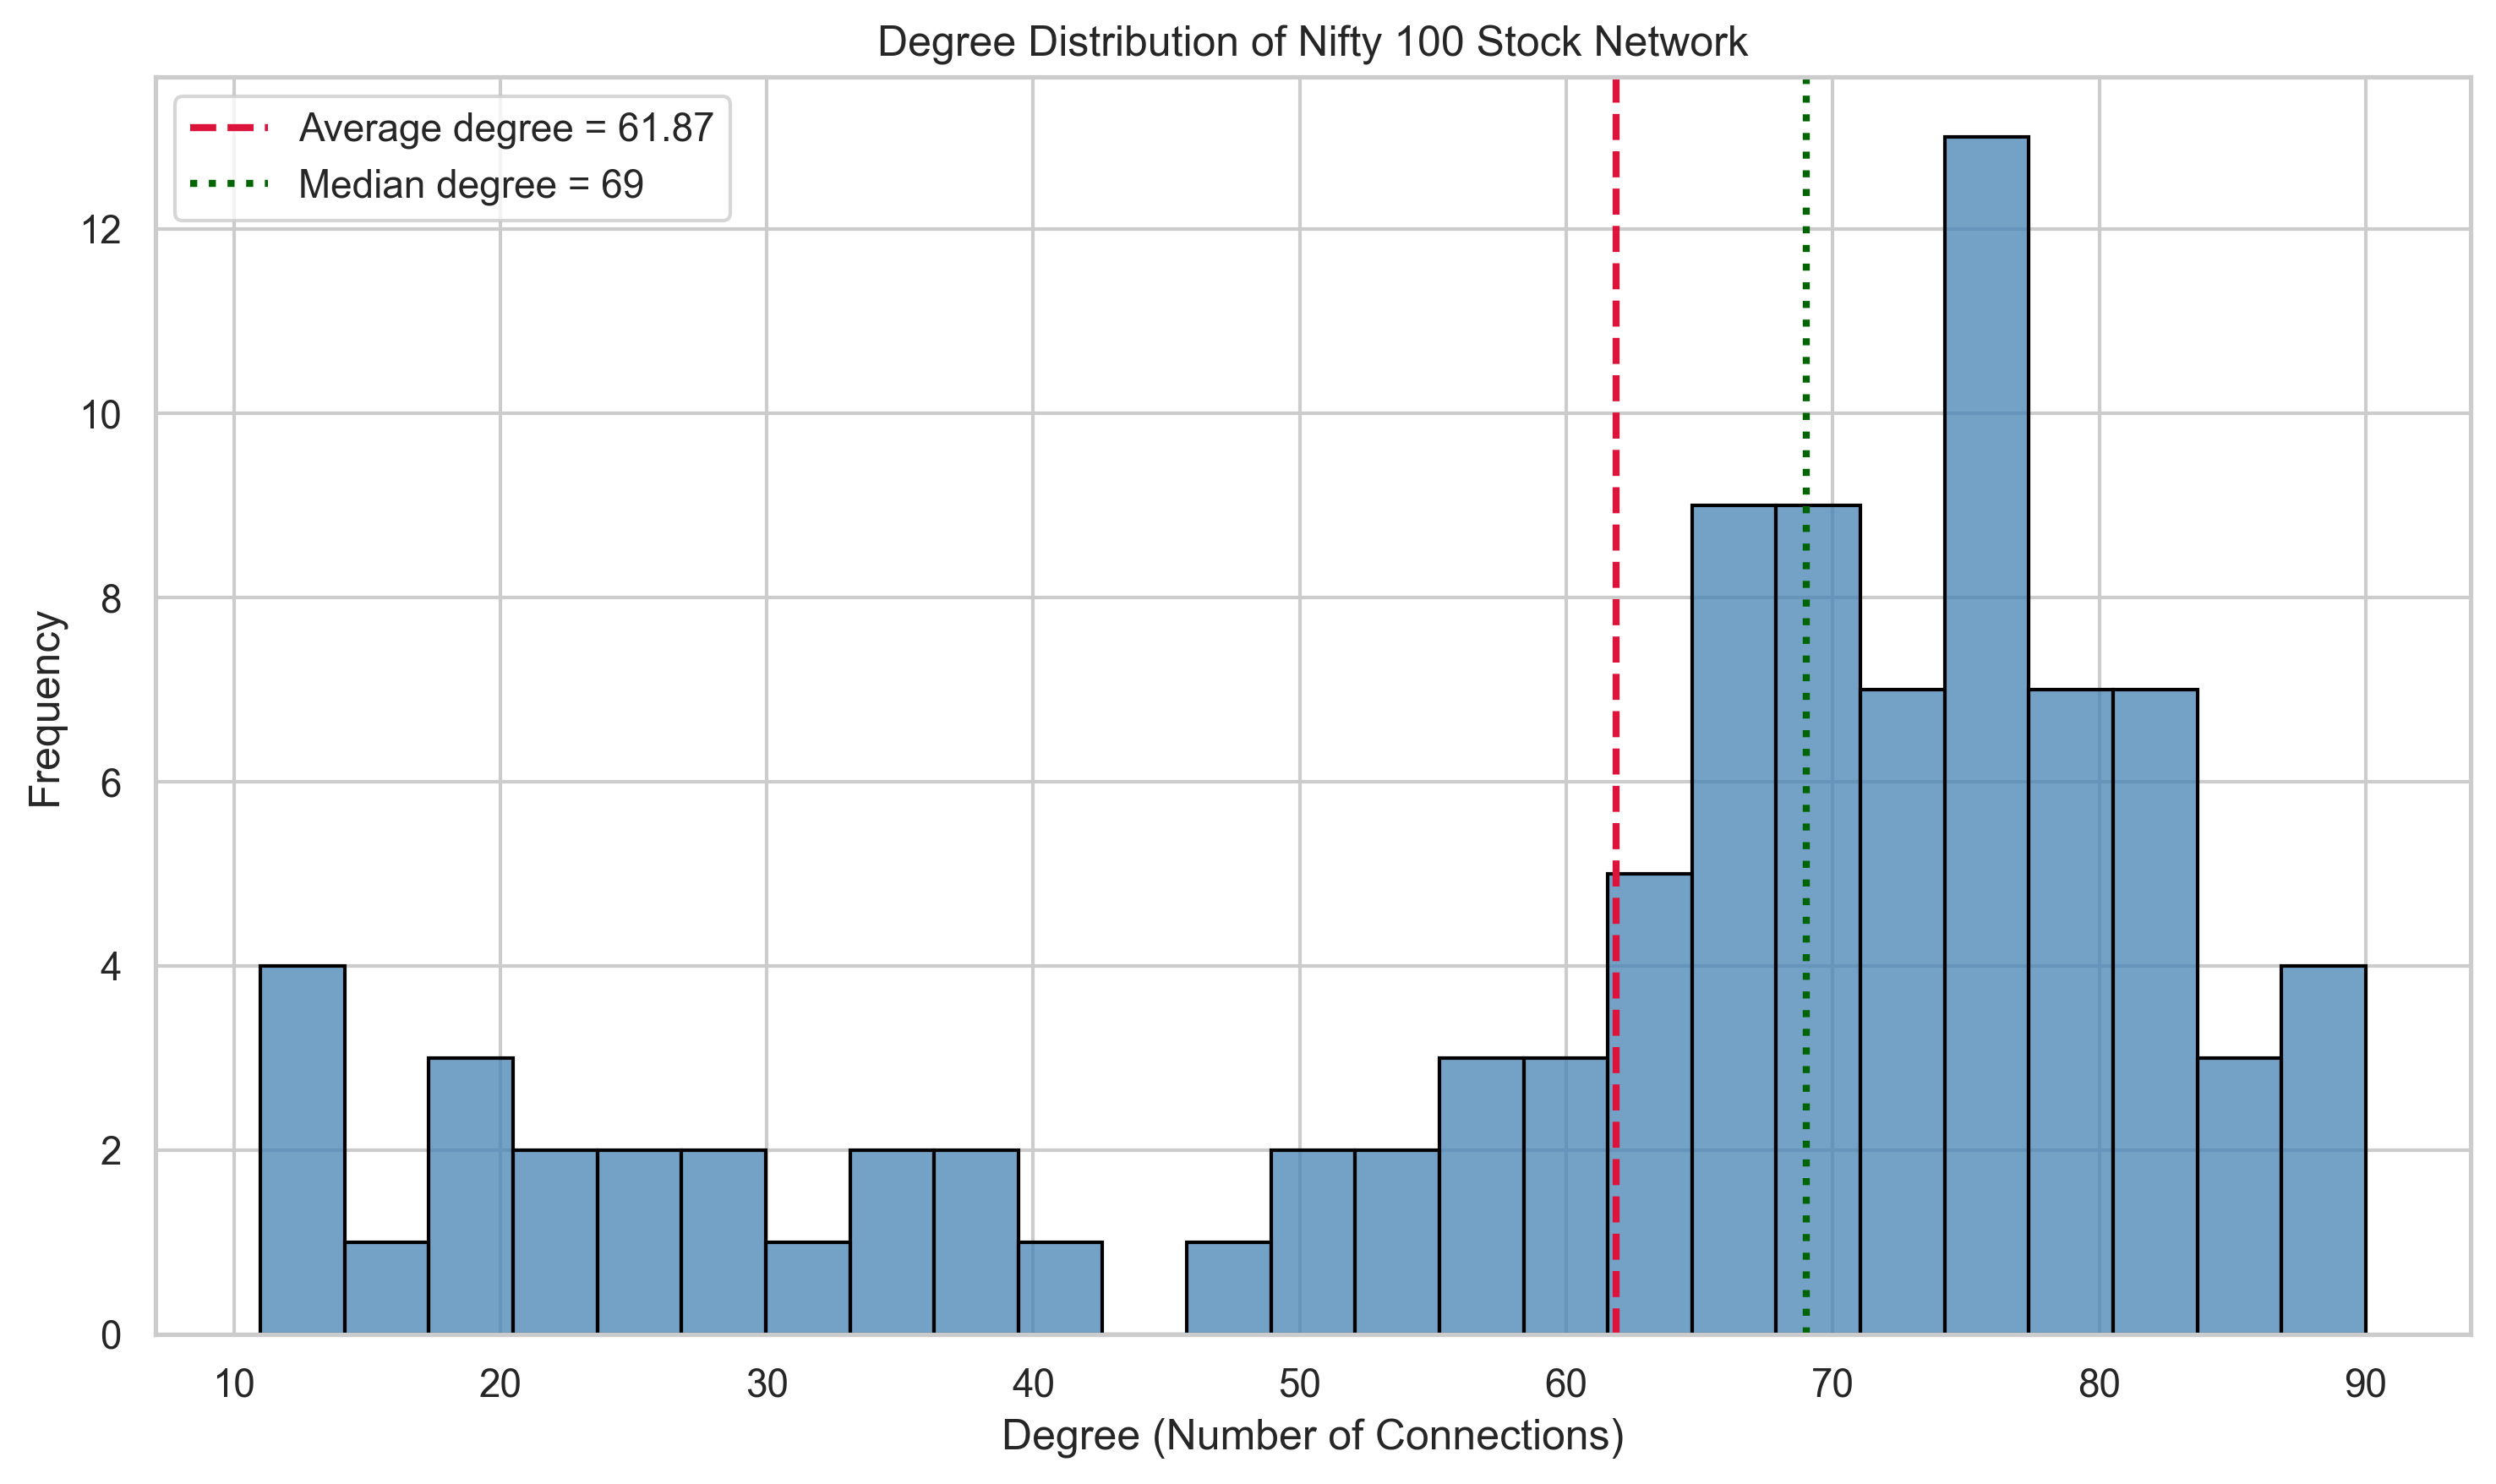
\includegraphics[width=\textwidth]{degree_histogram.png}
    \caption{Degree distribution.}
  \end{subfigure}
  \hfill
  \begin{subfigure}[t]{0.48\textwidth}
    \centering
    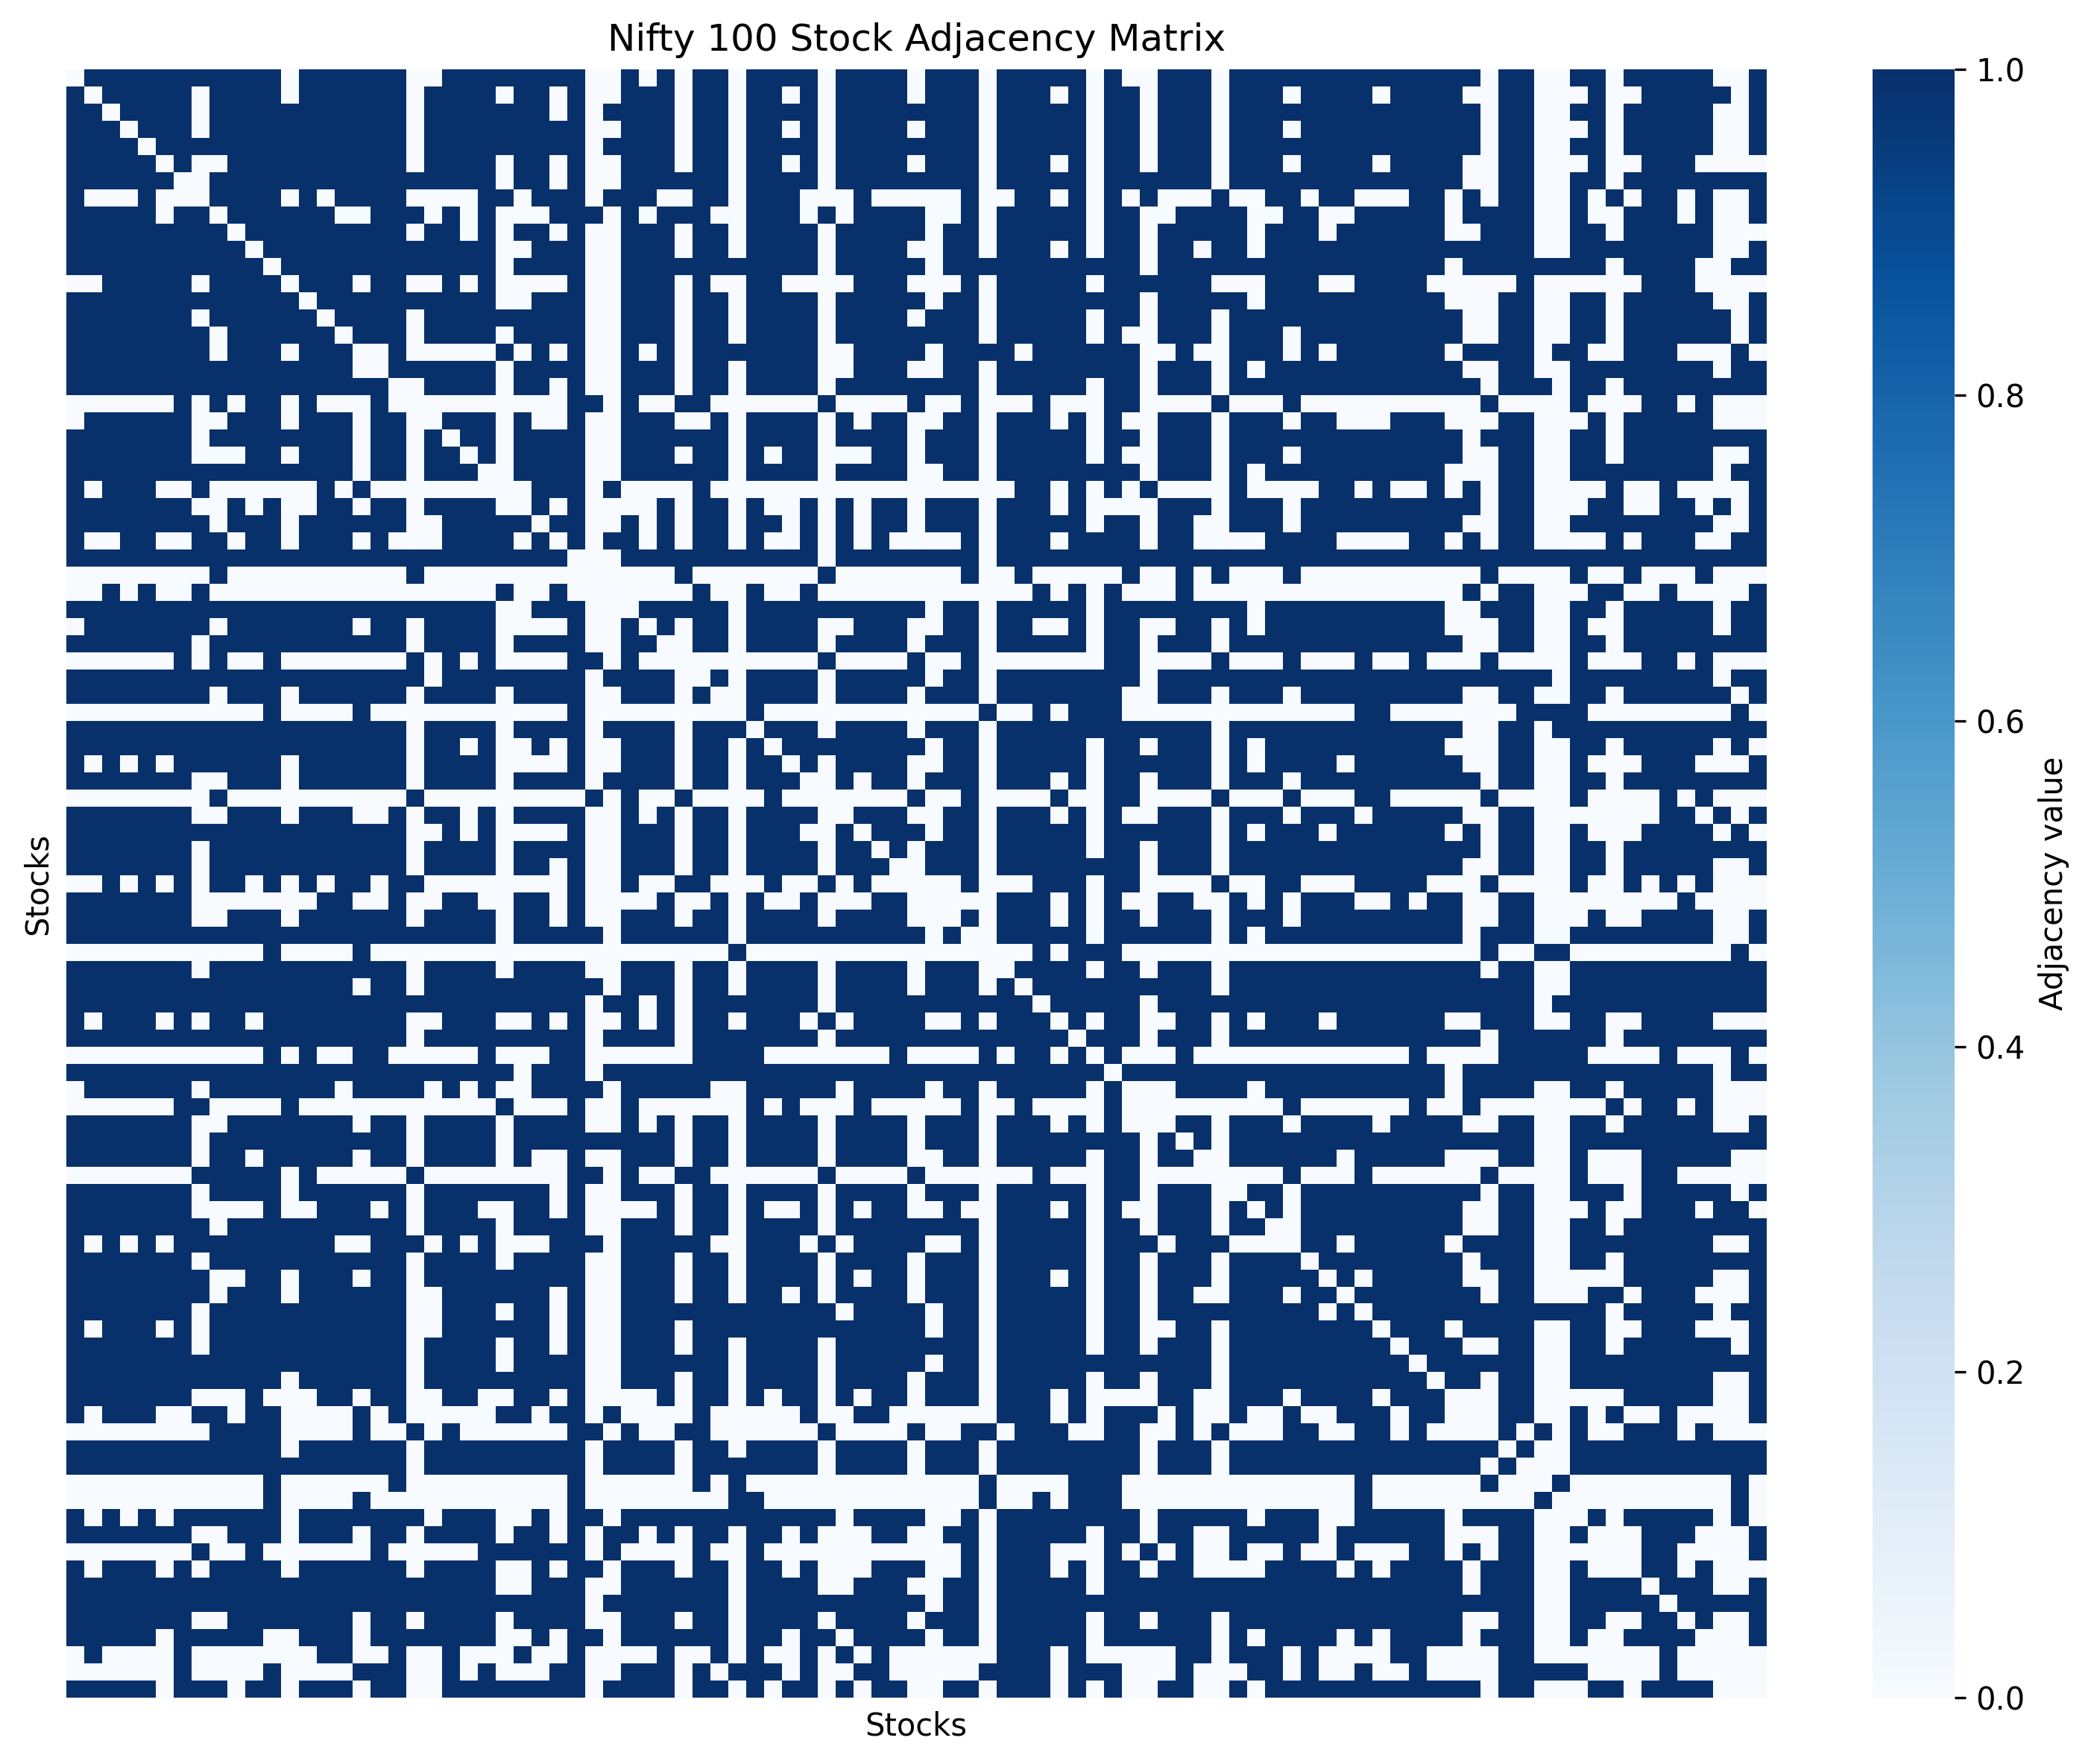
\includegraphics[width=\textwidth]{adjacency_matrix_heatmap.png}
    \caption{Binary adjacency matrix.}
  \end{subfigure}
  \caption{Degree distribution and adjacency structure of the main
  Nifty 100 network. The histogram includes average and median degree
  reference lines.}
\end{figure}

\resultfigure{degree_log_log_distribution.png}{0.82}
{Degree-frequency distribution on log--log axes.}

The log--log plot does not by itself establish a power law. In particular, a
straight-looking segment over a limited range is not sufficient evidence of a
scale-free network. The observed high density and relatively narrow
high-degree concentration are more consistent with broad market co-movement
at the selected low threshold than with a network dominated by a very small
number of hubs.

\subsection{Centrality Leaderboard}
The highest degree-centrality stocks are \texttt{DLF.NS} and
\texttt{M\&M.NS}. Other high-ranking stocks include
\texttt{ULTRACEMCO.NS} and \texttt{JSWSTEEL.NS}. These stocks also appear
near the top of the eigenvector-centrality ranking. This suggests that their
large number of connections is not limited to weakly connected peripheral
nodes.

\begin{table}[H]
\centering
\caption{Top five stocks for each centrality measure.}
\small
\begin{tabular}{llll}
\toprule
Rank & Degree & Betweenness & Eigenvector \\
\midrule
1 & DLF.NS & M\&M.NS & DLF.NS \\
2 & M\&M.NS & DLF.NS & ULTRACEMCO.NS \\
3 & ULTRACEMCO.NS & JSWSTEEL.NS & JSWSTEEL.NS \\
4 & JSWSTEEL.NS & LT.NS & M\&M.NS \\
5 & LT.NS & BAJAJFINSV.NS & LT.NS \\
\bottomrule
\end{tabular}
\end{table}

\resultfigure{top10_centrality_leaderboard.png}{0.98}
{Top-ten leaderboard for degree, betweenness, and eigenvector centrality.}

The betweenness ranking is similar but not identical to the degree ranking.
This distinction is important: a node can have many connections without
occupying a particularly strategic position between other parts of the
network. \texttt{M\&M.NS} has the largest betweenness score, while \texttt{RELIANCE.NS} also appears among the leading bridge-like
nodes. These results identify structural positions in the correlation graph,
they should not be interpreted as evidence that the stocks cause market
movements or are automatically superior investments.

\subsection{Clustering and Sector Homophily}
The average clustering coefficient is 0.849. The highest individual
coefficients include \texttt{VEDL.NS} (1.000), \texttt{POWERINDIA.NS}
(0.997), and \texttt{BSE.NS} (0.965). A high average means that many pairs of
neighbors of a stock are also connected, producing dense local triangles.

\resultfigure{top15_clustering_coefficients.png}{0.82}
{Fifteen stocks with the highest local clustering coefficients. The red line
shows the network-wide average.}

The sector assortativity coefficient is 0.021, which is close to zero. Thus,
after accounting for the observed sector labels, the network provides only
weak evidence that edges preferentially join stocks from the same sector.
Sector membership may still influence individual relationships, but the
thresholded correlations are also affected by market-wide factors and common
investor behavior.

\resultfigure{nifty100_network_by_industry_sector.png}{0.82}
{Plot for the main Nifty 100 network with nodes colored by sector. The low
assortativity indicates that sector membership alone does not explain most of
the observed connections.}

\subsection{Threshold Sensitivity}
The threshold results show a strong transition from a dense connected network
to a fragmented network. At threshold 0.1 there are 94,234 edges and one
connected component. At threshold 0.5, only 923 edges remain and the network
has 280 connected components. At threshold 0.9, there is only one edge and
446 components.

\begin{table}[H]
\centering
\caption{Selected threshold-sensitivity results.}
\small
\begin{tabular}{rrrrr}
\toprule
$\tau$ & Edges & Density & Avg. degree & Components \\
\midrule
0.1 & 94234 & 0.945 & 421.63 & 1 \\
0.2 & 63119 & 0.633 & 282.41 & 2 \\
0.3 & 23219 & 0.233 & 103.89 & 32 \\
0.4 & 4994 & 0.050 & 22.34 & 133 \\
0.5 & 923 & 0.009 & 4.13 & 280 \\
0.6 & 179 & 0.002 & 0.80 & 360 \\
0.7 & 50 & 0.001 & 0.22 & 411 \\
0.8 & 15 & $<0.001$ & 0.07 & 435 \\
0.9 & 1 & $<0.001$ & 0.00 & 446 \\
\bottomrule
\end{tabular}
\end{table}

\resultfigure{threshold_metrics.png}{0.88}
{Network properties as a function of the correlation threshold.}

The threshold-sensitivity calculation uses the saved
\texttt{correlation\_matrix.csv}, which contains 447 stocks, whereas the main
visualization and node-level results use the 95-node Nifty 100 adjacency
matrix. Consequently, the table and figure should be interpreted as a
Nifty 500-scale sensitivity experiment rather than as an exact re-evaluation
of the 95-node main network. This difference is a limitation of the current
pipeline and should be removed in a future version by generating and using a
separate Nifty 100 correlation matrix for the sensitivity analysis.

\section{Discussion}
The main network is dense at the selected threshold. This is expected when
absolute correlations are thresholded at a relatively permissive value:
common market movements allow many stocks to satisfy the edge condition.
Consequently, a high degree should be interpreted as broad historical
co-movement.

The similarity between the degree and eigenvector rankings suggests that the
most connected stocks are also embedded in the dense core of the network.
Betweenness adds a different perspective by identifying nodes that connect
otherwise less directly related portions of the graph. The high clustering
coefficient further indicates that strong relationships are not randomly
scattered, but rather form tightly-knit groups. Neighboring stocks tend to share many of their own neighbors.

The near-zero sector assortativity is an important counterpoint to the visual
presence of sector colors. The network appears to be influenced more strongly
by broad market co-movement than by strict industry boundaries. This result
may also reflect the use of absolute correlations, which combines positive
and negative relationships, and the use of an unweighted threshold that
discards the magnitude difference between correlations above the threshold.

\subsection{Economic Reality Check}
The network results are broadly consistent with how the Indian equity market
works. The Nifty 100 contains large
and actively traded companies. These companies are exposed to common forces
such as changes in interest rates, inflation, crude-oil prices, exchange rates,
global risk sentiment, domestic economic growth, and foreign-investor flows.
It is therefore economically reasonable that many stocks move together and
that the network is dense at a relatively low threshold.

The results also have a sector interpretation. Indian companies do
not operate in complete isolation: banks lend to companies in other sectors,
energy and commodity prices affect manufacturing and transport, and large
companies are held by many of the same domestic and foreign investors. These
links can create cross-sector correlations. The low sector assortativity
($0.021$) therefore does not mean that sectors are irrelevant. It means that,
in this sample and time window, sector membership alone does not explain most
of the edges. Broad market factors appear to be at least as important as
within-sector similarity.

% The centrality results are also economically plausible, but they should not be
% overinterpreted.
Stocks such as \texttt{RELIANCE.NS}, \texttt{HDFCBANK.NS},
\texttt{ICICIBANK.NS}, and \texttt{TCS.NS} are economically important large
companies and would be natural candidates for influential nodes in an Indian
market network. However, the highest scores in this particular calculation
include \texttt{DLF.NS}, \texttt{M\&M.NS}, \texttt{ULTRACEMCO.NS}, and
\texttt{JSWSTEEL.NS}. This difference is not necessarily an error. Centrality
is determined by correlation patterns during the chosen period, whereas
economic importance is also determined by market capitalization, revenues,
employment, index weights, and real-economy activity. A stock can be a
correlation hub without being the largest company in India. The use of log
returns may also contribute to this difference: they measure percentage-like
price movements and reduce the influence of price levels and compounding,
so the resulting correlations reflect co-movement in returns rather than
similarity in company size or absolute price changes. Different return
definitions, sampling frequencies, or volatility conditions could therefore
produce somewhat different centrality rankings. In addition, the adjacency
matrix is unweighted: once a correlation exceeds the threshold, its exact
magnitude is discarded. This may also contribute to differences between the
network rankings and economic reality, since weak and very strong links are
treated identically.

% The threshold results provide another reality check. At $|\rho|\geq0.2$, the
% network is highly connected because ordinary market-wide co-movement is enough
% to create many edges. At higher thresholds, only unusually strong
% relationships remain and the network fragments quickly. This is realistic:
% stocks often respond to the same broad news, but very strong co-movement is
% usually limited to particular periods, industries, or shocks.

Overall, the results match the broad economic reality of an integrated Indian
stock market: common shocks connect many sectors, while a smaller number of
relationships remain exceptionally strong. They do not, however, measure
causal influence, company quality, future returns, or the real-time state of
the Indian economy. A stronger economic comparison would require time-varying
networks, market-capitalization weights, sector indices, and macroeconomic
variables such as interest rates, inflation, exchange rates, and crude-oil
prices.

\section{Limitations and Future Work}
\begin{itemize}
  \item Correlation measures association and does not establish causation.
  \item The network is unweighted, so correlations of different strengths
  above the threshold are treated identically.
  \item The analysis uses a single historical window; relationships may vary
  across market regimes.
  \item The threshold-sensitivity experiment uses a 447-stock correlation
  matrix while the main graph uses 95 stocks.
  \item Sector labels are taken from the current constituent list and may not
  represent historical sector classifications throughout the entire period.
  \item Future work could compare positive-only and absolute correlations,
  use weighted networks, test rolling windows, and report largest-component
  size and average path length explicitly.
\end{itemize}

\section{Conclusion}
This project demonstrates how a stock market can be studied using network
science. The 95-node Nifty 100 network at $|\rho|\geq0.2$ is dense, highly
clustered, and organized around a broad group of well-connected stocks rather
than a single isolated hub. Degree, betweenness, and eigenvector centrality
highlight related but distinct structural roles. The low sector assortativity
indicates that stocks are not substantially more likely to be connected to
stocks from the same sector than to stocks from other sectors. Thus, the
observed links reflect broad market co-movement rather than only
within-sector similarity. Finally, threshold
sensitivity shows that the apparent connectivity of the market depends
strongly on how an edge is defined: raising the threshold removes edges and
quickly fragments the graph.

\begin{thebibliography}{9}
\bibitem{chi2010network}
K. Chi Tse, J. Liu, and F. C. M. Lau,
\newblock A network perspective of the stock market,
\newblock \emph{Journal of Empirical Finance}, 17(4):659--667, 2010.

\bibitem{moghadam2019complex}
H. E. Moghadam et al.,
\newblock Complex networks analysis in Iran stock market: The application of
centrality,
\newblock \emph{Physica A: Statistical Mechanics and its Applications},
531:121800, 2019.

\bibitem{newman2018}
M. E. J. Newman,
\newblock \emph{Networks: An Introduction},
\newblock 2nd ed., Oxford University Press, 2018.
\end{thebibliography}

\end{document}
